\begin{figure}
\begin{center}

\begin{subfigure}[b]{0.5\linewidth}
\centering
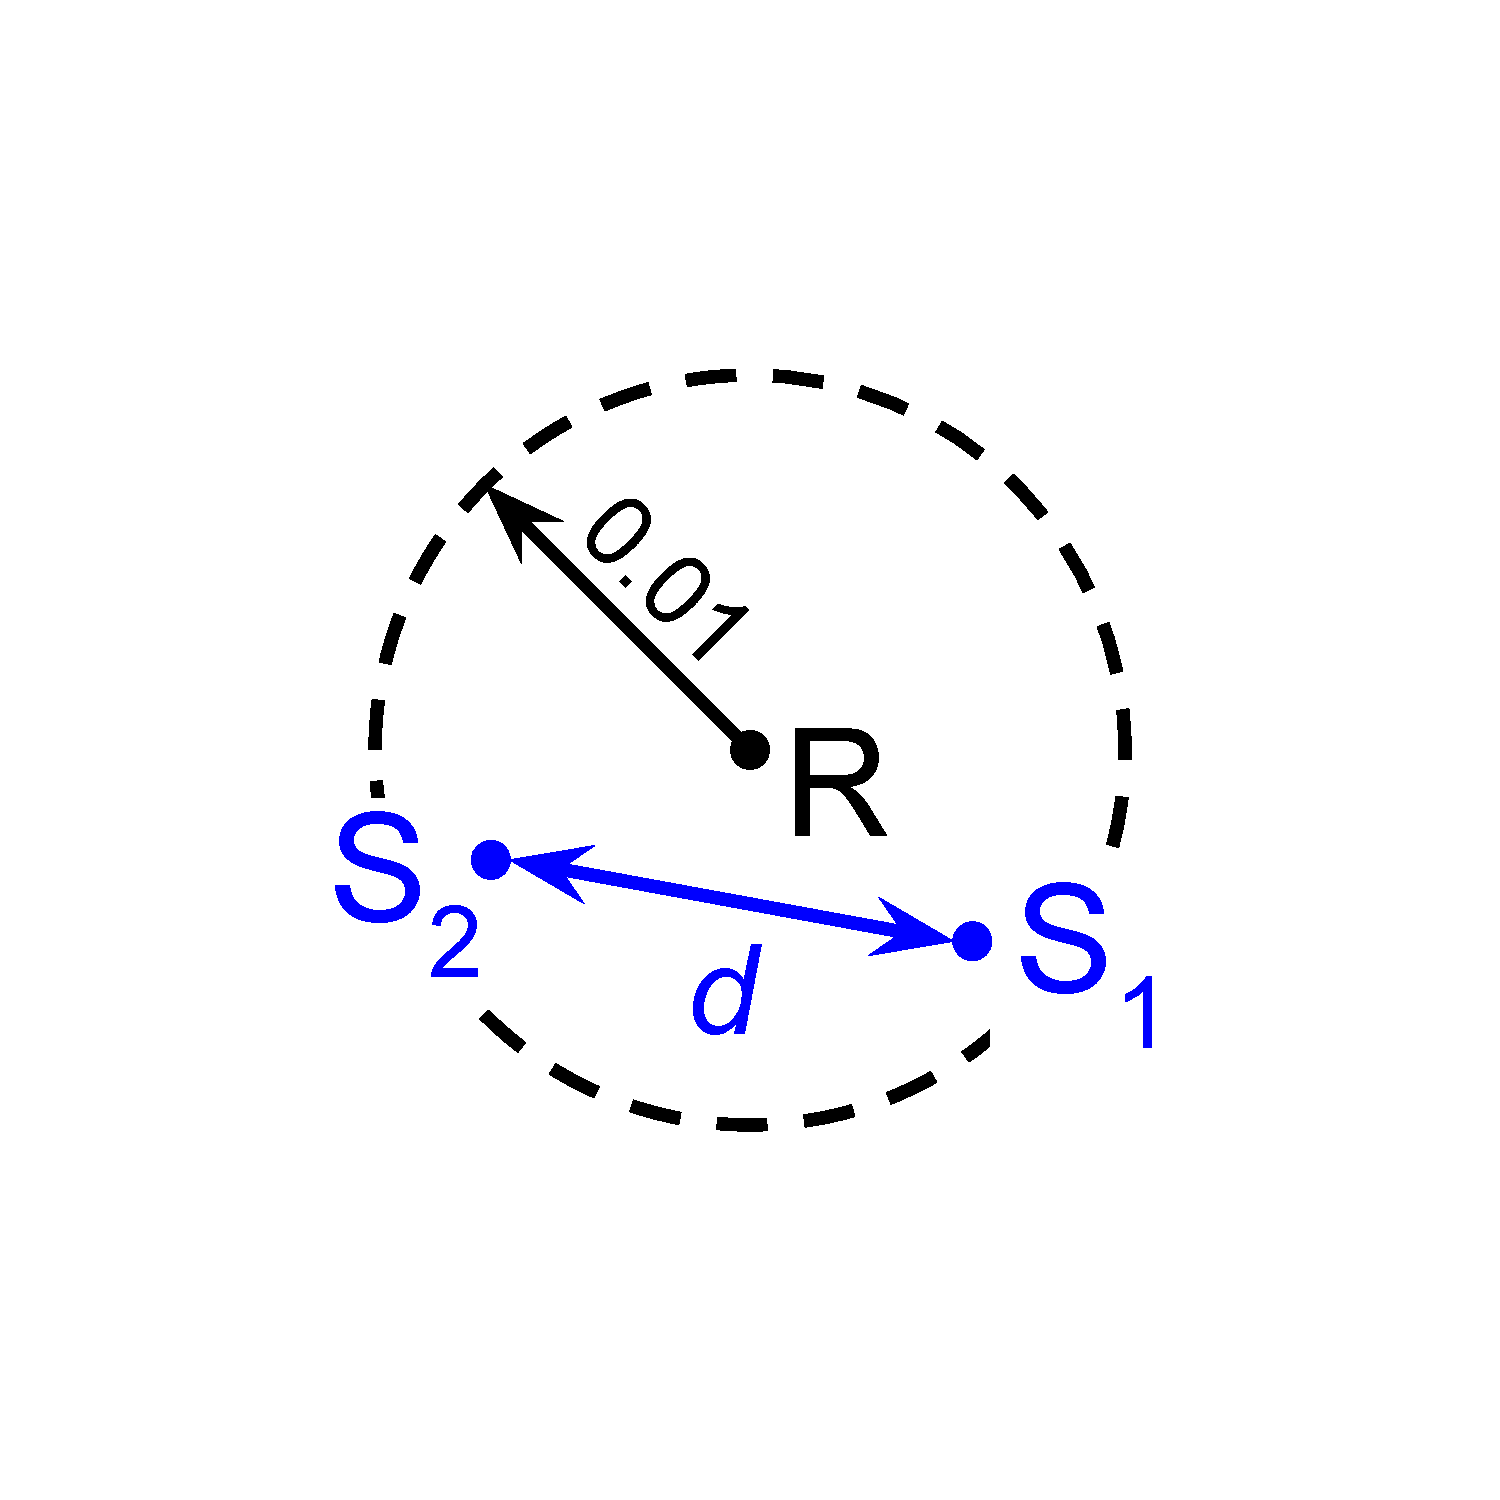
\includegraphics[width=\linewidth]{dimensionality-statistic}
\caption{
Dimensionality statistic
}
\label{fig:dimensionality_statistic}
\end{subfigure}%
\begin{subfigure}[b]{0.5\linewidth}
\centering
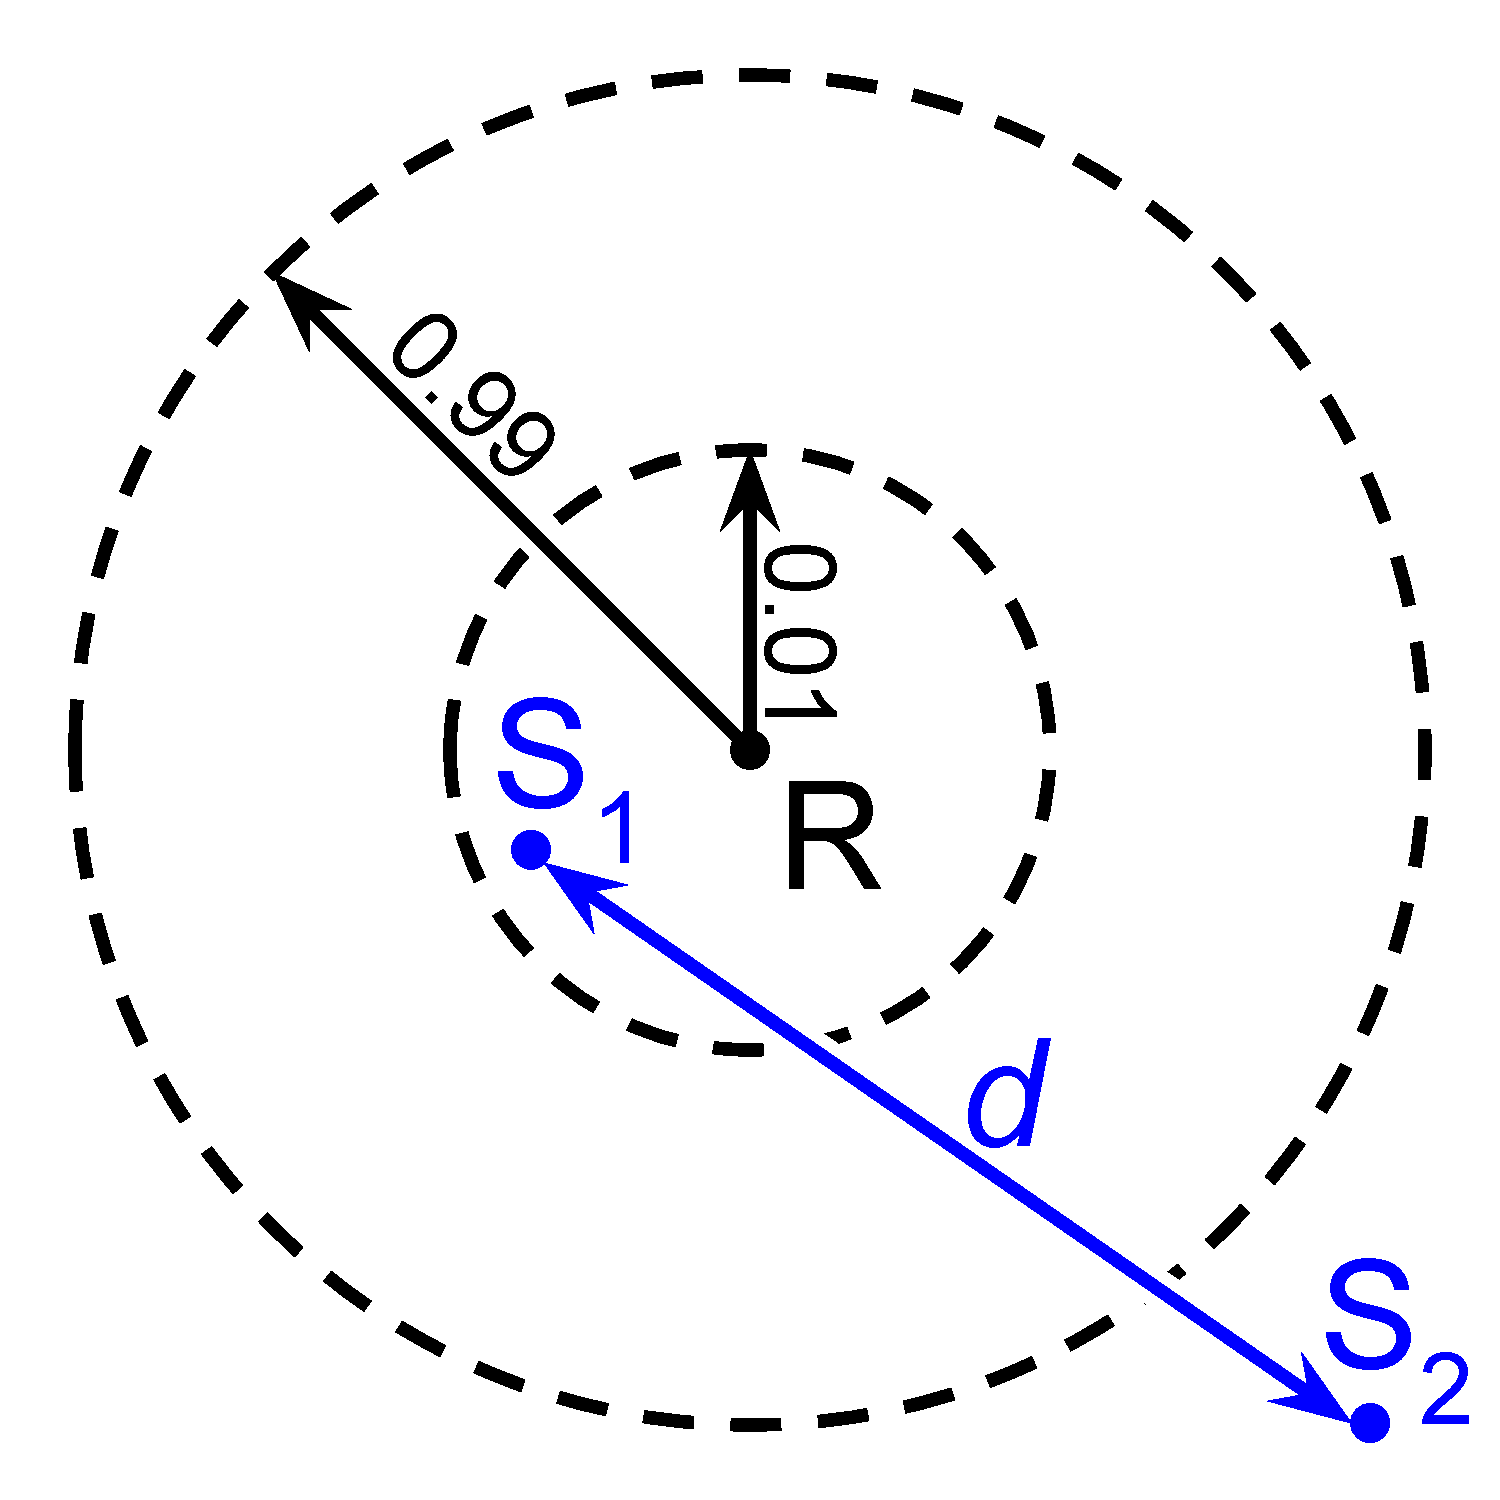
\includegraphics[width=\linewidth]{elasticity-statistic}
\caption{
Elsaticity statistic
}
\label{fig:elasticity_statistic}
\end{subfigure}

\caption{
A schematic depicting (A) the process used to generate the dimensionality statistic for each metric and (B) the process used to generate the elasticity statistic for each metric.
}
\label{fig:dimensionality_measure}

\end{center}
\end{figure}
